
%% bare_conf_compsoc.tex
%% V1.4b
%% 2015/08/26
%% by Michael Shell
%% See:
%% http://www.michaelshell.org/
%% for current contact information.
%%
%% This is a skeleton file demonstrating the use of IEEEtran.cls
%% (requires IEEEtran.cls version 1.8b or later) with an IEEE Computer
%% Society conference paper.
%%
%% Support sites:
%% http://www.michaelshell.org/tex/ieeetran/
%% http://www.ctan.org/pkg/ieeetran
%% and
%% http://www.ieee.org/

%%*************************************************************************
%% Legal Notice:
%% This code is offered as-is without any warranty either expressed or
%% implied; without even the implied warranty of MERCHANTABILITY or
%% FITNESS FOR A PARTICULAR PURPOSE! 
%% User assumes all risk.
%% In no event shall the IEEE or any contributor to this code be liable for
%% any damages or losses, including, but not limited to, incidental,
%% consequential, o_diagramr any other damages, resulting from the use or misuse
%% of any information contained here.
%%
%% All comments are the opinions http://www.bibtex.org/Using/of their respective authors and are not
%% necessarily endorsed by the IEEE.
%%
%% This work is distributed under the LaTeX Project Public License (LPPL)
%% ( http://www.latex-project.org/ ) version 1.3, and may be freely used,
%% distributed and modified. A copy of the LPPL, version 1.3, is included
%% in the base LaTeX documentation of all distributions of LaTeX released
%% 2003/12/01 or later.
%% Retain all contribution notices and credits.
%% ** Modified files should be clearly indicated as such, including  **
%% ** renaming them and changing author support contact information. **
%%*************************************************************************


% *** Authors should verify (and, if needed, correct) their LaTeX system  ***
% *** with the testflow diagnostic prior to trusting their LaTeX platform ***
% *** with production work. The IEEE's font choices and paper sizes can   ***
% *** trigger bugs that do not appear when using other class files.       ***                          ***
% The testflow support page is at:
% http://www.michaelshell.org/tex/testflow/



\documentclass[conference,compsoc]{IEEEtran}
% Some/most Computer Society conferences require the compsoc mode option,
% but others may want the standard conference format.
%
% If IEEEtran.cls has not been installed into the LaTeX system files,
% manually specify the path to it like:
% \documentclass[conference,compsoc]{../sty/IEEEtran}





% Some very useful LaTeX packages include:
% (uncomment the ones you want to load)


% *** MISC UTILITY PACKAGES ***
%
%\usepackage{ifpdf}
% Heiko Oberdiek's ifpdf.sty is very useful if you need conditional
% compilation based on whether the output is pdf or dvi.
% usage:
% \ifpdf
%   % pdf code
% \else
%   % dvi code
% \fi
% The latest version of ifpdf.sty can be obtained from:
% http://www.ctan.org/pkg/ifpdf
% Also, note that IEEEtran.cls V1.7 and later provides a builtin
% \ifCLASSINFOpdf conditional that works the same way.
% When switching from latex to pdflatex and vice-versa, the compiler may
% have to be run twice to clear warning/error messages.






% *** CITATION PACKAGES ***
%
\ifCLASSOPTIONcompsoc
  % IEEE Computer Society needs nocompress option
  % requires cite.sty v4.0 or later (November 2003)
  \usepackage[nocompress]{cite}
\else
  % normal IEEE
  \usepackage{cite}
\fi
% cite.sty was written by Donald Arseneau
% V1.6 and later of IEEEtran pre-defines the format of the cite.sty package
% \cite{} output to follow that of the IEEE. Loading the cite package will
% result in citation numbers being automatically sorted and properly
% "compressed/ranged". e.g., [1], [9], [2], [7], [5], [6] without using
% cite.sty will become [1], [2], [5]--[7], [9] using cite.sty. cite.sty's
% \cite will automatically add leading space, if needed. Use cite.sty's
% noadjust option (cite.sty V3.8 and later) if you want to turn this off
% such as if a citation ever needs to be enclosed in parenthesis.
% cite.sty is already installed on most LaTeX systems. Be sure and use
% version 5.0 (2009-03-20) and later if using hyperref.sty.
% The latest version can be obtained at:
% http://www.ctan.org/pkg/cite
% The documentation is contained in the cite.sty file itself.
%
% Note that some packages require special options to format as the Computer
% Society requires. In particular, Computer Society  papers do not use
% compressed citation ranges as is done in typical IEEE papers
% (e.g., [1]-[4]). Instead, they list every citation separately in order
% (e.g., [1], [2], [3], [4]). To get the latter we need to load the cite
% package with the nocompress option which is supported by cite.sty v4.0
% and later.





% *** GRAPHICS RELATED PACKAGES ***
%
\renewcommand{\figurename}{Fig.}
\ifCLASSINFOpdf
  \usepackage[pdftex]{graphicx}
  % declare the path(s) where your graphic files are
  \graphicspath{{../schematics/svg/}{../schematics/imagenes/}}
  % and their extensions so you won't have to specify these with
  % every instance of \includegraphics
  \DeclareGraphicsExtensions{.pdf,.jpeg,.png}
\else
  % or other class option (dvipsone, dvipdf, if not using dvips). graphicx
  % will default to the driver specified in the system graphics.cfg if no
  % driver is specified.
  % \usepackage[dvips]{graphicx}
  % declare the path(s) where your graphic files are
  % \graphicspath{{../eps/}}
  % and their extensions so you won't have to specify these with
  % every instance of \includegraphics
  % \DeclareGraphicsExtensions{.eps}
\fi
% graphicx was written by David Carlisle and Sebastian Rahtz. It is
% required if you want graphics, photos, etc. graphicx.sty is already
% installed on most LaTeX systems. The latest version and documentation
% can be obtained at: 
% http://www.ctan.org/pkg/graphicx
% Another good source of documentation is "Using Imported Graphics in
% LaTeX2e" by Keith Reckdahl which can be found at:
% http://www.ctan.org/pkg/epslatex
%
% latex, and pdflatex in dvi mode, support graphics in encapsulated
% postscript (.eps) format. pdflatex in pdf mode supports graphics
% in .pdf, .jpeg, .png and .mps (metapost) formats. Users should ensure
% that all non-photo figures use a vector format (.eps, .pdf, .mps) and
% not a bitmapped formats (.jpeg, .png). The IEEE frowns on bitmapped formats
% which can result in "jaggedy"/blurry rendering of lines and letters as
% well as large increases in file sizes.
%
% You can find documentation about the pdfTeX application at:
% http://www.tug.org/applications/pdftex





% *** MATH PACKAGES ***
%
\usepackage{amsmath}
% A popular package from the American Mathematical Society that provides
% many useful and powerful commands for dealing with mathematics.
%
% Note that the amsmath package sets \interdisplaylinepenalty to 10000
% thus preventing page breaks from occurring within multiline equations. Use:
\interdisplaylinepenalty=2500
% after loading amsmath to restore such page breaks as IEEEtran.cls normally
% does. amsmath.sty is already installed on most LaTeX systems. The latest
% version and documentation can be obtained at:
% http://www.ctan.org/pkg/amsmath





% *** SPECIALIZED LIST PACKAGES ***
%
\usepackage{algorithmic}
% algorithmic.sty was written by Peter Williams and Rogerio Brito.
% This package provides an algorithmic environment fo describing algorithms.
% You can use the algorithmic environment in-text or within a figure
% environment to provide for a floating algorithm. Do NOT use the algorithm
% floating environment provided by algorithm.sty (by the same authors) or
% algorithm2e.sty (by Christophe Fiorio) as the IEEE does not use dedicated
% algorithm float types and packages that provide these will not provide
% correct IEEE style captions. The latest version and documentation of
% algorithmic.sty can be obtained at:
% http://www.ctan.org/pkg/algorithms
% Also of interest may be the (relatively newer and more customizable)
% algorithmicx.sty package by Szasz Janos:
% http://www.ctan.org/pkg/algorithmicx




% *** ALIGNMENT PACKAGES ***
%
\usepackage{array}
% Frank Mittelbach's and David Carlisle's array.sty patches and improves
% the standard LaTeX2e array and tabular environments to provide better
% appearance and additional user controls. As the default LaTeX2e table
% generation code is lacking to the point of almost being broken with
% respect to the quality of the end results, all users are strongly
% advised to use an enhanced (at the very least that provided by array.sty)
% set of table tools. array.sty is already installed on most systems. The
% latest version and documentation can be obtained at:
% http://www.ctan.org/pkg/array


% IEEEtran contains the IEEEeqnarray family of commands that can be used to
% generate multiline equations as well as matrices, tables, etc., of high
% quality.




% *** SUBFIGURE PACKAGES ***
\ifCLASSOPTIONcompsoc
  \usepackage[caption=false,font=footnotesize,labelfont=sf,textfont=sf]{subfig}
\else
  \usepackage[caption=false,font=footnotesize]{subfig}
\fi
% subfig.sty, written by Steven Douglas Cochran, is the modern replacement
% for subfigure.sty, the latter of which is no longer maintained and is
% incompatible with some LaTeX packages including fixltx2e. However,
% subfig.sty requires and automatically loads Axel Sommerfeldt's caption.sty
% which will override IEEEtran.cls' handling of captions and this will result
% in non-IEEE style figure/table captions. To prevent this problem, be sure
% and invoke subfig.sty's "caption=false" package option (available since
% subfig.sty version 1.3, 2005/06/28) as this is will preserve IEEEtran.cls
% handling of captions.
% Note that the Computer Society format requires a sans serif font rather
% than the serif font used in traditional IEEE formatting and thus the need
% to invoke different subfig.sty package options depending on whether
% compsoc mode has been enabled.
%
% The latest version and documentation of subfig.sty can be obtained at:
% http://www.ctan.org/pkg/subfig




% *** FLOAT PACKAGES ***
%
%\usepackage{fixltx2e}
% fixltx2e, the successor to the earlier fix2col.sty, was written by
% Frank Mittelbach and David Carlisle. This package corrects a few problems
% in the LaTeX2e kernel, the most notable of which is that in current
% LaTeX2e releases, the ordering of single and double column floats is not
% guaranteed to be preserved. Thus, an unpatched LaTeX2e can allow a
% single column figure to be placed prior to an earlier double column
% figure.
% Be aware that LaTeX2e kernels dated 2015 and later have fixltx2e.sty's
% corrections already built into the system in which case a warning will
% be issued if an attempt is made to load fixltx2e.sty as it is no longer
% needed.
% The latest version and documentation can be found at:
% http://www.ctan.org/pkg/fixltx2e


%\usepackage{stfloats}
% stfloats.sty was written by Sigitas Tolusis. This package gives LaTeX2e
% the ability to do double column floats at the bottom of the page as well
% as the top. (e.g., "\begin{figure*}[!b]" is not normally possible in
% LaTeX2e). It also provides a command:
%\fnbelowfloat
% to enable the placement of footnotes below bottom floats (the standard
% LaTeX2e kernel puts them above bottom floats). This is an invasive package
% which rewrites many portions of the LaTeX2e float routines. It may not work
% with other packages that modify the LaTeX2e float routines. The latest
% version and documentation can be obtained at:
% http://www.ctan.org/pkg/stfloats
% Do not use the stfloats baselinefloat ability as the IEEE does not allow
% \baselineskip to stretch. Authors submitting work to the IEEE should note
% that the IEEE rarely uses double column equations and that authors should try
% to avoid such use. Do not be tempted to use the cuted.sty or midfloat.sty
% packages (also by Sigitas Tolusis) as the IEEE does not format its papers in
% such ways.
% Do not attempt to use stfloats with fixltx2e as they are incompatible.
% Instead, use Morten Hogholm'a dblfloatfix which combines the features
% of both fixltx2e and stfloats:
%
% \usepackage{dblfloatfix}
% The latest version can be found at:
% http://www.ctan.org/pkg/dblfloatfix




% *** PDF, URL AND HYPERLINK PACKAGES ***
%
%\usepackage{url}
% url.sty was written by Donald Arseneau. It provides better support for
% handling and breaking URLs. url.sty is already installed on most LaTeX
% systems. The latest version and documentation can be obtained at:
% http://www.ctan.org/pkg/url
% Basically, \url{my_url_here}.




% *** Do not adjust lengths that control margins, column widths, etc. ***
% *** Do not use packages that alter fonts (such as pslatex).         ***
% There should be no need to do such things with IEEEtran.cls V1.6 and later.
% (Unless specifically asked to do so by the journal or conference you plan
% to submit to, of course. )

% correct bad hyphenation here
\usepackage{amssymb}
\hyphenation{op-tical net-works semi-conduc-tor}


\begin{document}
%
% paper title
% Titles are generally capitalized except for words such as a, an, and, as,
% at, but, by, for, in, nor, of, on, or, the, to and up, which are usually
% not capitalized unless they are the first or last word of the title.
% Linebreaks \\ can be used within to get better formatting as desired.
% Do not put math or special symbols in the title.
%\title{Bare Demo of IEEEtran.cls for\\ IEEE Computer Society Conferences}
\title{Arquitectura de Hardware para Convoluci\'on Bidimensional\\ con Memoria
  Limitada Aplicada al Procesamiento de Im\'agenes}


% author names and affiliations
% use a multiple column layout for up to three different
% affiliations
\author{\IEEEauthorblockN{Martin Casabella,
  Sergio Sulca,
  Ivan Vignolles
}
\IEEEauthorblockA{Escuela de Ingenier\'ia en Computaci\'on\\
  Facultad de Ciencias Exactas F\'isicas y Naturales\\
  Universidad Nacional de C\'ordoba\\
  Email: martin.casabella@gmail.com, ser.0090@gmail.com, ivignolles@alumnos.unc.edu.ar}
}
% conference papers do not typically use \thanks and this command
% is locked out in conference mode. If really needed, such as for
% the acknowledgment of grants, issue a \IEEEoverridecommandlockouts
% after \documentclass

% for over three affiliations, or if they all won't fit within the width
% of the page (and note that there is less available width in this regard for
% compsoc conferences compared to traditional conferences), use this
% alternative format:
% 
%\author{\IEEEauthorblockN{Michael Shell\IEEEauthorrefmark{1},
%Homer Simpson\IEEEauthorrefmark{2},
%James Kirk\IEEEauthorrefmark{3}, 
%Montgomery Scott\IEEEauthorrefmark{3} and
%Eldon Tyrell\IEEEauthorrefmark{4}}
%\IEEEauthorblockA{\IEEEauthorrefmark{1}School of Electrical and Computer Engineering\\
%Georgia Institute of Technology,
%Atlanta, Georgia 30332--0250\\ Email: see http://www.michaelshell.org/contact.html}
%\IEEEauthorblockA{\IEEEauthorrefmark{2}Twentieth Century Fox, Springfield, USA\\
%Email: homer@thesimpsons.com}
%\IEEEauthorblockA{\IEEEauthorrefmark{3}Starfleet Academy, San Francisco, California 96678-2391\\
%Telephone: (800) 555--1212, Fax: (888) 555--1212}
%\IEEEauthorblockA{\IEEEauthorrefmark{4}Tyrell Inc., 123 Replicant Street, Los Angeles, California 90210--4321}}




% use for special paper notices
%\IEEEspecialpapernotice{(Invited Paper)}




% make the title area
\maketitle

% As a general rule, do not put math, special symbols or citations
% in the abstract
\begin{abstract}
  En este art\'iculo se presenta una arquitectura de hardware para realizar una
  convoluci\'on 2D en una FPGA cuando no se puede instanciar suficiente memoria
  RAM para poder alojar la imagen completa. Se prioriz\'o la velocidad de
  procesamiento, el uso eficiente de los recursos y un dise\~no escalable donde
  se pudieran agregar tantas operaciones de convoluci\'on en paralelo como se
  desee sin deber hacer grandes modificaciones en el dise\~no.
\end{abstract}

% no keywords




% For peer review papers, you can put extra information on the cover
% page as needed:
% \ifCLASSOPTIONpeerreview
% \begin{center} \bfseries EDICS Category: 3-BBND \end{center}
% \fi
%
% For peerreview papers, this IEEEtran command inserts a page break and
% creates the second title. It will be ignored for other modes.
\IEEEpeerreviewmaketitle



\section{Introducci\'on}
La convoluci\'on bidimensional discreta es ampliamente usada en múltiples campos de la
ingenieria, siendo uno de ellos la visi\'on artificial que ha tomado fuerza en la
ultima d\'ecada con los resultados obtenidos con las redes neuronales
convolucionales. El creciente tama\~no en los modelos, como tambien en la
informacion disponible para el entrenamiento hacen de la velocidad de
procesamiento un factor de gran importancia.

Por la naturaleza de los datos y de la operaci\'on de la convoluci\'on, un enfoque
paralelo resulta mucho m\'as eficiente que uno secuencial en lo que a velocidad de
procesamiento respecta. Se utilizaron FPGAs para la implementacion, pues
resuelven la necesidad de paralelismo como tambi\'en la de poder
probar distintos prototipos de arquitecturas de hardware.

La convoluci\'on discreta en 2D esta definida por la siguiente
ecuaci\'on: 

\begin{equation}\label{conv-org}
S(x,y) = \sum_{i} \sum_{j}I(x-i,y-j)K(i, j)
\end{equation}

Al no ser necesaria la propiedad de conmutatividad en este caso, es posible
eliminar el proceso de espejar una de las matrices\cite{Goodfellow-et-al-2016} ,
obteniendo la funci\'on de correlacion cruzada

\begin{equation}\label{conv}
S(x,y) = \sum_{i} \sum_{j}I(x+i,y+j)K(i, j)
\end{equation}

la cual ser\'a en realidad  implementada, por lo que en lo que resta
del art\'iculo, cada vez que se nombre a la operaci\'on de convoluci\'on,
se estar\'a haciendo referencia a la ecuaci\'on \ref{conv}.

Uno de los mayores desaf\'ios fue trabajar con memoria RAM lo suficientemente
escaza que no fuera capaz de alojar todos los pixels de la imagen que se desea
procesar. Por lo que la im\'agen debe ser fraccionada y procesada en lotes, con
todo el procesamiento adicional que esto implica.

Por una cuesti\'on de simplicidad, todo el trabajo se desarroll\'o utilizando
imagenes en escala de grises, al tener estas un \'unico canal.


\section{An\'alisis Previo}
The analysis purpose is work whit a finite minimum representation for image
pixels and kernel values. To that is necessary make a study about bits number for
a god image representation.

Pixels values \(I_{ij}\) have a range from 0 to 255. We use normalization
dynamic range expansion\cite{dinamic_rango} in ordet to get a new range from
0 to 1. Kernel values \(K_{ij}\) can to be negative or positive. Thus We use
Maximum norm\cite{max_norm} to get maximum absolute value then it 
divide to every \(K_{ij}\) to achieve a new range from -1 to 1. So kernel
effect is maintain. 

We use Signed Fixed Point representation\cite{fix_p} \(S(8,7)\) in order to use
previos ranges.

Convolution of image whit a kernel  $\mathbb{K}^{3{\times}3}$ results in 20-bits
output \(S(20,14)\). Hence we make post-processing. It come result value to
positive range and truncate value. We compare both output post-processing and
20-bits so that find a minimum bits amount and do not lose important data. 

We use SNR measure between ouput 20-bits \(S(20,14)\) and error that results from
reduce bits number \(e_r=f(x)_{20b}-f(x)_{pos}\)\cite{srntesis}. Representation
\(S(13,8)\) has a approximate SNR \(30 [dB]\) that show filter effect whit minimum
data loss. It is acceptable becouse the objet in no show a perfect image.

The values can come to a 8-bits representatio using dynamic range
expansion\cite{dinamic_rango} but it se need to get  maximum and minimum
number pixel value after convolution. So image should be in memory totally.

\section{Design and implementation}

\subsection{Workflow}
As shown in figure \ref{fig_workflow}, the workflow consists of three
instances: first, in the PC a python script does the preprocessing 
described in section \ref{preproc}, separates the image in batches and then sends the kernel's
coefficients and the first batch through an UART connection to the FPGA. In the
FPGA a microprocessor receives the information and communicates it to the
convolution module using a 32 bits GPIO port. The batch is then convolved with
the kernel inside the module. When the operation is finished a notification is
sent to the microprocessor, which gives the order to retrieve the processed batch
from the module and sends it to the PC and then waits for the next batch to arrive.

\begin{figure}[!t]
\centering
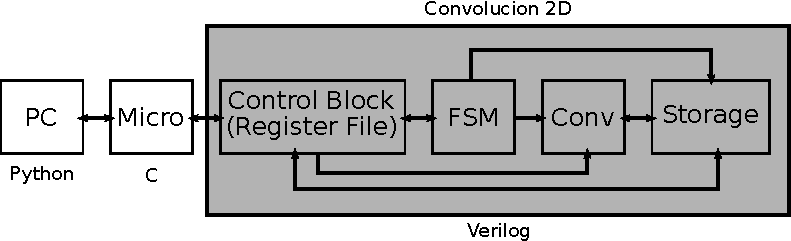
\includegraphics[width=3in]{workflow}
\caption{System's workflow and languages used in every instance}
\label{fig_workflow}
\end{figure}

\subsection{Convolution Module}
The module was designed with three objectives: fast pixel processing rate,
efficient use of the memory and parallel processing scalability.

The module's architecture is shown in figure \textbf{REFERENCIAAIMAGENQUEFALTA},
the \textbf{control unit} is the one in charge of handling the communication
with the processor, in the \textbf{convolution unit} is where the sum of
the products of the kernel's coefficients with the pixels happen, the
\textbf{address generation unit (AGU)} manages the memory addresses, the
\textbf{memory management unit (MMU)} manages how the values in memory must be
read and written, and finally the \textbf{storage}, which is implemented with a
set of columns of the FPGA's block RAM.

\subsubsection{States}
It is possible to see that during the work cycle, the convolution module goes
through several states, as shown in figure \ref{state}.

At the beginning the module must be in a \textbf{reset} state, waiting to be
configured, to do so the most significant bit of the 32 bits input in the module
must be set to high. The figure \textbf{FIGURABITS} shows the 32 bits input
frame structure and the binary code for the instructions.

The module will stay in the \textbf{reset} state until it receives the
instruction to go to the \textbf{KernelLoad} state, in which state the kernel
coefficients are loaded into the module. Then it goes to the \textbf{SizeLoad}
state where the image's height is loaded, the need for this is explained in
section \ref{infstorage}. Once the module has gone through this setup states it
will not come back to them until the entire image is processed. Now the
processing loop start, first the module goes to the \textbf{ImageLoad} state and
saves in the memory the batch, then is goes to the \textbf{Run} state where the
processing occurs, while in processing the module can not be interrupted, i.e.
it will ignore all instructions till the batch is processed, as soon as the
processing is ended a notification will be emitted through Control Unit's
\textit{EoP} pin and the module will wait the instruction to got to the
\textbf{Out} state where the already processed batch is send back to the microprocessor.

All this states logic is managed by the control unit, which depending on the
state will communicate the corresponding control signal to the other components
of the module.

\begin{figure}[!t]
  \centering
  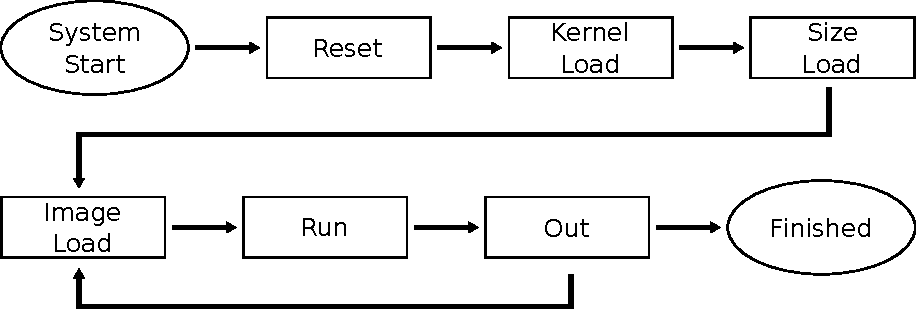
\includegraphics[width=2.5in]{states.pdf}
  \caption{Diagrama de estados del m\'odulo de convoluci\'on.
    A - Carga de kernel, B - Carga de tama\~no, C - Carga de imagen, D -
    Procesamiento, E - Out, F - Reset}
  \label{state}
\end{figure}

\subsubsection{Data storage}\label{infstorage}
The kernel coefficients are stored in registers inside each convolution unit. In
order to store a batch, the proposed approach is to arrange the block RAM memory
in columns, where each of them will store a image's pixel column. Therefore a
batch size is given by the height of the image and the number of memory columns,
also the maximum height of the image will be restricted by the number of entries
that each memory columns has.

During a batch processing, every pixel is read only once, so in order to do a
more efficient use of the memory, the pixels that were already used are
overwritten with processed pixels. This approach reduces drastically the amount
of memory needed because it reuses the same memory to store the input batch and the
processed batch. In the section \ref{dataproc} additional aspects of the design
that reduces even more the memory use are explained.

\subsubsection{Data processing}\label{dataproc}
Given a $k\times k$ kernel, each convolution unit takes $k$ adjacent memory columns as
input. To produce the first processed pixel, a convolution unit first needs to
load $k$ pixels from each columns in such a way as to have $k\times
k$ pixels loaded into it, then proceeds to multiply the pixels with the kernel's
coefficients and sum everything. Finally, it truncates the result to reduce the
bit length and the result is saved into the first position of the memory.

Once a pixel is processed, it is saved into the memory while the convolution unit
shifts its image register, discarding the oldest $k$ pixels and loading new $k$
pixels, i.e. one from each input column, like a FIFO structure. As shown in
figure \ref{proc_conv}, this procedure is equivalent to shit the kernel
vertically on the image. All this procedure is synchronized in such a way that
one processed pixel is generated in every clock cycle.

The AGU manages the memory's read and write address, it takes into account the
latency between the clock cycle where the first pixel in the memory is read and
the clock cycle where the first processed pixel is written in memory. This latency is
equal to $k$ plus some more clock cycles needed to latch values during the
convolution, and the difference between the read address and the write address
must be equal to it.

\begin{figure}[!t]
\centering
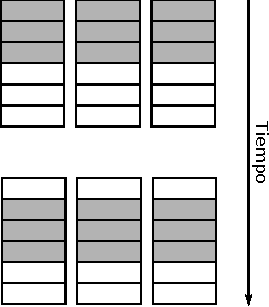
\includegraphics[width=2.5in]{proc_conv.pdf}
\caption{En gris se observan los datos que han sido cargados a los registros del
bloque de convoluci\'on, en el ciclo siguiente es posible ver como los valores
de cada columna que ingresaron primero han sido decartados, y nuevos valores han
sido cargados, produciendo un efecto de desplazamiento hacia abajo.}
\label{proc_conv}
\end{figure}

Until this point the analysis was over a single convolution unit, now the
approach to work with multiple convolution units working in parallel is
described.

As mentioned above, $k$ columns are needed as input to produce one processed
column in a convolution unit, that means that $2k$ columns are needed for two
convolution units, however given the nature of the convolution operation, to
produce a contiguous column it is necessary to shift the input columns by one.
Hence, there is an overlap between the two inputs and this produces that even that $k$ input columns are still needed per convolution unit, only
$k+1$ different input columns are needed. For that reason, it was decided that
multiple convolution units in parallel will produce contiguous processed
columns, sharing the common input columns. With this approach, for $N$
convolution units the number of memory columns needed gets reduced from $N\cdot
k$ to $N+k-1$.

\textbf{IMAGEN DE OVERLAP}

The same overlap explained above produces also that repeated data will be needed
between one batch and the next one. In order to eliminate the need to send data
that already is in the memory, an algorithm was designed. Given $N$ convolution
units and a $k\times k$ kernel, a $N+k-1$ batch width is needed, but the
processed batch has a width of $N$ columns, i.e. one for each convolution unit,
therefore the last $k-1$ memory columns are not overwritten and maintain the
input data. This $k-1$ columns will be reused as the first columns of the 
next batch, thus the batch width is reduced to $N$, with the exception of
the first batch that will still have a $N+k-1$ width.

A consequence of reusing the memory columns written by the previous batch is
that in every iteration the position of the memory columns associated with each
convolution unit describes a circular shift by $N$ places. From the above it
follows that a periodicity in the relation between the memory columns and the
convolution units' inputs must exist, where the period $It$ is the number of
iterations necessary to get to the original memory columns - convolution units
inputs relation, i.e. when $It(k-1)$ is a multiple of $N+k-1$. That is, there
must be an integer $m$ such that 

\begin{equation}\label{niter}
  \frac{It}{m} = \frac{N}{k-1} + 1
\end{equation}

\textbf{AGREGAR CUADRITO DE ALGORITMO CON CARGA, PROCESAMIENTO Y SALIDA}
The algorithm is implemented in the MMU, which serves as an interface between
the memories and the rest of the components, keeping them independent from the
level of parallelism and the iteration number.

%\section{Arquitectura del sistema}
%
%\subsection{Flujo de trabajo}
%El flujo de trabajo consta de tres instancias como se observa en la figura
%\ref{fig_workflow}. En la primer instancia, se desarroll\'o un cliente en python
%donde se ingresa la imagen a procesar junto con los coeficientes del filtro que
%se desea aplicar, el filtro o kernel es una matriz que pertence al conjunto
%$\mathbb{R}^{3{\times}3}$. Toda la arquitectura del sistema ha sido dise\~nada
%para trabajar con filtros de esa dimensi\'on, aunque no deber\'ia ser dificil
%generalizarla a filtros de otras dimensiones.
%\begin{figure}[!t]
%\centering
%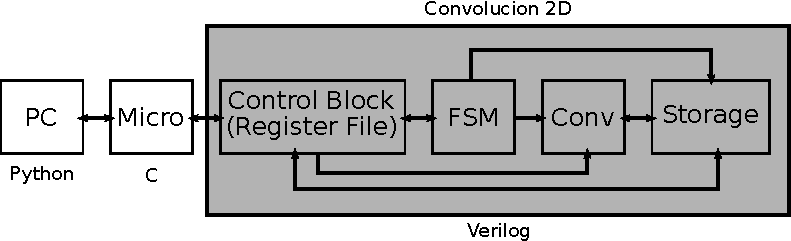
\includegraphics[width=3in]{workflow.pdf}
%\caption{Flujo de trabajo del sistema y lenguajes en los que se trabaj\'o en
%  cada instancia.}
%\label{fig_workflow}
%\end{figure}
%La informaci\'on es entonces separada en lotes, el cliente env\'ia un
%lote, espera a recibir el mismo procesado y luego env\'ia el lote siguiente.
%
%Un microprocesador instanciado en la FPGA es el encargado de recibir los lotes,
%hace un desempaquetado de los datos y adem\'as le a\~nade a los mismos una 
%cabecera necesaria para la comunicaci\'on con el m\'odulo de convoluci\'on.
%Asimismo una vez que el m\'odulo finaliz\'o el procesamiento, el microprocesador 
%toma esa informaci\'on procesada, la empaqueta y env\'ia nuevamente a la
%computadora.
%
%El m\'odulo de convoluci\'on procesa el lote, internamente es el Bloque de
%Control (Control Block) quien hace de interfaz entre el resto del m\'odulo y el
%exterior. La porci\'on de la imagen es almacenada, los bloques de convoluci\'on
%(Conv) realizan la suma de los productos de los coeficientes del filtro con una
%secci\'on de la imagen igual al tama\~no del filtro, una vez que toda la
%porci\'on de la imagen fue procesada, se env\'ia el resultado y se espera a
%recibir una nueva porci\'on. Una maquina de estados finitos (FSM) lleva cuenta
%del ciclo de entrada$\rightarrow$procesamiento$\rightarrow$salida que ocurre en
%el m\'odulo.
%
%\subsection{M\'odulo de convoluci\'on}
%En esta secci\'on se describe en detalle la arquitectura del m\'odulo de
%convoluci\'on.
%
%\subsubsection{Estados}
%Durante todo el ciclo de trabajo, el m\'odulo atraviesa distintos estados como
%se aprecia en la figura \ref{state}. En primera instancia, est\'a en un estado
%inicial de \textbf{reset} esperando a ser configurado. Permanecer\'a en ese
%estado hasta recibir la intruccion para pasar al estado de \textbf{kernel load}
%(carga de kernel) donde se carga al m\'odulo el filtro que se desea aplicar. Una
%vez que se termina de cargar los coeficientes 
%del filtro, se espera la instrucci\'on para pasar a \textbf{size load} (carga
%de tama\~no), en este estado se debe informar al m\'odulo la altura de la
%imagen. Habiendo ocurrido la transici\'on al estado siguiente, no se retornar\'a
%a los estados previos hasta finalizar el procesamiento completo de la imagen.
%Al salir del estado de \textbf{size load} se pasa al de \textbf{image load}
%donde se carga una secci\'on de la imagen. Pasados estos tres estados se
%finaliza la etapa de carga. En la instacia siguiente el m\'odulo se encuentra en
%el estado de \textbf{run}. En este estado se realiza el procesamiento del lote
%de forma ininterrumpida, es decir, toda instrucci\'on ser\'a ignorada hasta
%finalizar el filtrado donde una se\~nal de aviso es emitida. Se espera entonces
%la instrucci\'on para pasar al estado \textbf{out}. Con el lote ya procesado y
%la intrucci\'on recibida se da inicio al env\'io de los datos filtrados. La
%sucesi\'on de los ultimos tres estados mensionados \textbf{image load}
%$\rightarrow$ \textbf{run} $\rightarrow$ \textbf{out} se repetir\'a por cada
%nuevo lote hasta obtener la imagen procesada en su totalidad.
%
%
%\subsubsection{Almacenamiento de la informaci\'on}
%El kernel o filtro que se quiere aplicar a la imagen es almacenado en registros de los bloques de convoluci\'on. Con
%respecto a la imagen, se opt\'o por ordenar la memoria en columnas, donde cada
%columna almacena una columna de pixels. Queda entonces como una limitaci\'on la
%altura m\'axima de la imagen dada por el n\'umero m\'aximo de pixels que es
%posible almacenar en una columna de memoria.
%
%El lote ya procesado es almacenado sobreescribiendo los datos que se utilizaron
%para producirlo, es decir, se utiliza la misma memoria tanto para los datos de
%entrada como los de salida.
%
%\subsubsection{Procesamiento de la informaci\'on}
%Cada bloque de convoluci\'on toma los valores de tres (o $k$, para un filtro que
%pertence a $\mathbb{R}^{k{\times}k}$) columnas adyacentes. Comienza cargando los
%tres primeros valores de cada columna en sus registros, realiza la suma del
%producto con los coeficientes del filtro, y hace un 
%desplazamiento de los registros con los valores de la imagen, de forma que se
%descarten los valores mas antiguos de cada columna, y se cargue un nuevo valor
%por columna, como en una estructura FIFO (first in, first out). Como muestra
%la figura \ref{proc_conv}, esto es equivalente a ubicar el filtro sobre tres
%columnas de la imagen y desplazarlo verticalemente.
%
%\begin{figure}[!t]
%\centering
%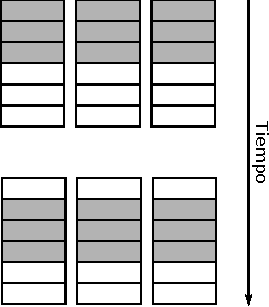
\includegraphics[width=2.5in]{proc_conv.pdf}
%\caption{En gris se observan los datos que han sido cargados a los registros del
%bloque de convoluci\'on, en el ciclo siguiente es posible ver como los valores
%de cada columna que ingresaron primero han sido decartados, y nuevos valores han
%sido cargados, produciendo un efecto de desplazamiento hacia abajo.}
%\label{proc_conv}
%\end{figure}
%
%Luego de analizar distintas alternativas, se decidi\'o que los bloques de
%convoluci\'on que se tienen trabajando en paralelo produzcan columnas procesadas
%contiguas, es decir, que el bloque de convoluci\'on 1 produzca la primer
%columna del lote, el bloque 2 la segunda y asi sucesivamente. Una de las
%razones por la que se tomo esta decisi\'on es la naturaleza de la operaci\'on de
%la convoluci\'on: se necesitan $k$ columnas de imagen para generar una columna procesada, para generar la
%columna contigua es necesario desplazarse un lugar en la imagen de entrada,
%por lo que existe unicamente una columna de diferencia en la entrada de dos
%bloques que generan dos columnas adyacentes. Esta superposici\'on en la entrada implica una
%reduccion del n\'umero de columnas necesarias de $k \cdot N$ a $N+k-1$ para N
%bloques de convoluci\'on si estos generan columnas adyacentes.


% An example of a floating figure using the graphicx package.
% Note that \label must occur AFTER (or within) \caption.
% For figures, \caption should occur after the \includegraphics.
% Note that IEEEtran v1.7 and later has special internal code that
% is designed to preserve the operation of \label within \caption
% even when the captionsoff option is in effect. However, because
% of issues like this, it may be the safest practice to put all your
% \label just after \caption rather than within \caption{}.
%
% Reminder: the "draftcls" or "draftclsnofoot", not "draft", class
% option should be used if it is desired that the figures are to be
% displayed while in draft mode.
%
%\begin{figure}[!t]
%\centering
%\includegraphics[width=2.5in]{myfigure}
% where an .eps filename suffix will be assumed under latex, 
% and a .pdf suffix will be assumed for pdflatex; or what has been declared
% via \DeclareGraphicsExtensions.
%\caption{Simulation results for the network.}
%\label{fig_sim}
%\end{figure}

% Note that the IEEE typically puts floats only at the top, even when this
% results in a large percentage of a column being occupied by floats.


% An example of a double column floating figure using two subfigures.
% (The subfig.sty package must be loaded for this to work.)
% The subfigure \label commands are set within each subfloat command,
% and the \label for the overall figure must come after \caption.
% \hfil is used as a separator to get equal spacing.
% Watch out that the combined width of all the subfigures on a 
% line do not exceed the text width or a line break will occur.
%
%\begin{figure*}[!t]
%\centering
%\subfloat[Case I]{\includegraphics[width=2.5in]{box}%
%\label{fig_first_case}}
%\hfil
%\subfloat[Case II]{\includegraphics[width=2.5in]{box}%
%\label{fig_second_case}}
%\caption{Simulation results for the network.}
%\label{fig_sim}
%\end{figure*}
%
% Note that often IEEE papers with subfigures do not employ subfigure
% captions (using the optional argument to \subfloat[]), but instead will
% reference/describe all of them (a), (b), etc., within the main caption.
% Be aware that for subfig.sty to generate the (a), (b), etc., subfigure
% labels, the optional argument to \subfloat must be present. If a
% subcaption is not desired, just leave its contents blank,
% e.g., \subfloat[].


% An example of a floating table. Note that, for IEEE style tables, the
% \caption command should come BEFORE the table and, given that table
% captions serve much like titles, are usually capitalized except for words
% such as a, an, and, as, at, but, by, for, in, nor, of, on, or, the, to
% and up, which are usually not capitalized unless they are the first or
% last word of the caption. Table text will default to \footnotesize as
% the IEEE normally uses this smaller font for tables.
% The \label must come after \caption as always.
%
%\begin{table}[!t]
%% increase table row spacing, adjust to taste
%\renewcommand{\arraystretch}{1.3}
% if using array.sty, it might be a good idea to tweak the value of
% \extrarowheight as needed to properly center the text within the cells
%\caption{An Example of a Table}
%\label{table_example}
%\centering
%% Some packages, such as MDW tools, offer better commands for making tables
%% than the plain LaTeX2e tabular which is used here.
%\begin{tabular}{|c||c|}
%\hline
%One & Two\\
%\hline
%Three & Four\\
%\hline
%\end{tabular}
%\end{table}


% Note that the IEEE does not put floats in the very first column
% - or typically anywhere on the first page for that matter. Also,
% in-text middle ("here") positioning is typically not used, but it
% is allowed and encouraged for Computer Society conferences (but
% not Computer Society journals). Most IEEE journals/conferences use
% top floats exclusively. 
% Note that, LaTeX2e, unlike IEEE journals/conferences, places
% footnotes above bottom floats. This can be corrected via the
% \fnbelowfloat command of the stfloats package.




\section{Conclusion}
The conclusion goes here.




% conference papers do not normally have an appendix



% use section* for acknowledgment
\ifCLASSOPTIONcompsoc
  % The Computer Society usually uses the plural form
  \section*{Acknowledgments}
\else
  % regular IEEE prefers the singular form
  \section*{Acknowledgment}
\fi


The authors would like to thank...





% trigger a \newpage just before the given reference
% number - used to balance the columns on the last page
% adjust value as needed - may need to be readjusted if
% the document is modified later
%\IEEEtriggeratref{8}
% The "triggered" command can be changed if desired:
%\IEEEtriggercmd{\enlargethispage{-5in}}

% references section

% can use a bibliography generated by BibTeX as a .bbl file
% BibTeX documentation can be easily obtained at:
% http://mirror.ctan.org/biblio/bibtex/contrib/doc/
% The IEEEtran BibTeX style support page is at:
% http://www.michaelshell.org/tex/ieeetran/bibtex/
%\bibliographystyle{IEEEtran}
% argument is your BibTeX string definitions and bibliography database(s)
%\bibliography{IEEEabrv,../bib/paper}
%
% <OR> manually copy in the resultant .bbl file
% set second argument of \begin to the number of references
% (used to reserve space for the reference number labels box)
\bibliographystyle{IEEEtran}
\bibliography{PROJECT_DOC}
%\begin{thebibliography}{1}
%
%\bibitem{IEEEhowto:kopka}
%H.~Kopka and P.~W. Daly, \emph{A Guide to \LaTeX}, 3rd~ed.\hskip 1em plus
  %0.5em minus 0.4em\relax Harlow, England: Addison-Wesley, 1999.
%
%\end{thebibliography}




% that's all folks
\end{document}


